\documentclass[dvipdfmx,11pt,a4paper,oneside,openany]{jsbook}
\usepackage{package}
%\usepackage{a4wide}
\usepackage[dvipdfmx]{hyperref}
\usepackage{pxjahyper}
\usepackage{tikz}
\usetikzlibrary{intersections, calc, arrows.meta}


%\addtolength{\fullwidth}{1truemm} %全体の幅(ヘッダ部の幅)を既定値から26mm小さくする
\setlength{\textwidth}{\fullwidth}  %本文の幅(textwidth)を全体の幅(=ヘッダ部の幅)にそろえる
\setlength{\evensidemargin}{5truemm}   %偶数ページの左余白を10mm(+1インチ)にする
\setlength{\oddsidemargin}{5truemm}    %奇数ページの左余白を10mm(+1インチ)にする

%\title{}
%\author{}
%\date{\today}
\begin{document}
%\maketitle

%\tableofcontents

%\makeatletter
%\@addtoreset{equation}{section}
%\def\theequation{\thesection.\arabic{equation}}
%\makeatother
\newcommand{\ctext}[1]{\raise0.2ex\hbox{\textcircled{\scriptsize{#1}}}}

% 表示文字列を"図"から"Figure"へ
\renewcommand{\figurename}{Fig. }

% 図番号を"<章番号>.<図番号>" へ
\renewcommand{\thefigure}{\arabic{figure}}

\setcounter{chapter}{4}
\chapter{QUANTISATION OF STATIC SOLUTION}
\section{Introduction}
これまでの議論では波動方程式から始まり, ミンコフスキー空間やユークリッド空間において, 様々なLocalizeされた古典解を調べ, 場の古典論との対応関係を調べてきた. 本チャプターではこれまで見てきた古典解に対して, 新たに場の量子論との関係を議論していく. %実際, 古典的なミンコフスキー解を量子論の束縛状態や散乱理論に関連付けることができたり, 励起状態を記述できたりする.

最もシンプルな方法として2章でメインに扱ったような静的ソリトン解の量子化から始めていくが, それにあたっては場の古典論と場の量子論の違いを把握した上で, その対応関係を通して議論が展開されていく. そのためにそれぞれの性質と対応関係について下記にまとめておく.

\vspace{1cm}
\begin{tikzpicture}
    \draw (2.9,5.7)--(2.9,6.3)--(4.8,6.3)--(4.8,5.7)--(2.9,5.7);
    \draw (2.9,6) node[right]{場の古典論};
    \draw (10.5,5.7)--(10.5,6.3)--(12.4,6.3)--(12.4,5.7)--(10.5,5.7);
    \draw (10.5,6) node[right]{場の量子論};
    \draw (0,0)--(15.2,0);
    \draw (0,0)--(0,6)--(2.9,6);
    \draw (4.8,6)--(10.5,6);
    \draw (12.4,6)--(15.2,6);
    \draw (15.2,0)--(15.2,6);
    \draw[dashed] (7.52,0)--(7.52,6);
    \draw (0.1,5) node[right]{1. 場が\underline{\bf c-numberの関数で記述}される.};
    \draw (7.6,5) node[right]{1. 場が\underline{\bf q-number(演算子)の関数で記述}される.};
    \draw (0.1,4.2) node[right]{2. 古典系において複数の\underline{\bf 場の状態の区別が可能}.};
    \draw (7.6,4.2) node[right]{2. 量子系において複数の\underline{\bf 場の状態の区別が不可能}.};
    \draw (7.9,3.8) node[right]{\footnotesize{$\rightarrow$ ヒルベルト空間においてSchr\"{o}dinger方程式に従う状態}};
    \draw (8.3,3.5) node[right]{\footnotesize{ベクトルを用いて区別.}};
    \draw (0.1,2.7) node[right]{3. 場のダイナミクスは\underline{\bf 非線形偏微分方程式}で記述};
    \draw (0.5,2.3) node[right]{され, \underline{\bf 解はスカラー関数}として現れる.};
    \draw (7.6,2.7) node[right]{3. 場のダイナミクスは\underline{\bf Heisenberg方程式で記述}};
    \draw (8,2.3) node[right]{され, \underline{\bf 解は演算子の関数}として現れる.};
    \draw (0.1,1.5) node[right]{4. 実際の\underline{\bf 粒子(particle)の概念を適用しない}.};
    \draw (0.4,1.1) node[right]{\footnotesize{$\rightarrow$ 粒子"描像"を適用.}};
    \draw (7.6,1.5) node[right]{4. 実際の\underline{\bf 粒子(particle)の概念が適用できる}.};
    \draw (7.9,1.1) node[right]{\footnotesize{$\rightarrow$ 同時固有状態にハミルトニアンと運動量演算子を作用させ}};
    \draw (8.2,0.8) node[right]{\footnotesize{た時, $E^2-\bm{P}^2=M^2$の関係から一定値$M$を生じる.}};
\end{tikzpicture}

%これらの手法の選択は、調和振動子の問題にシュレディンガー微分方程式、ファインマン経路積分、ハイゼンベルグ整流器法のどれを使うかというように、好みの問題もあります。

\section{The central idea}
一次元のポテンシャル$V(x)$に従う単位質量の粒子を考え, 古典論と量子論の比較をしながら, 量子化の手順を説明していく.

\subsection{How to describe the particle in classical theory and quantum theory}
古典論においてこの粒子を記述する際には運動方程式を用いて
\begin{align}
    \frac{\mathrm{d^2}x}{\mathrm{d^2}t}=-\frac{\mathrm{d}V}{\mathrm{d}x}
\end{align}
で与えられ, その運動は$x(t)$で記述される. 一方, 量子論では粒子を記述するのに, $x$を用いるのではなく, 粒子の各エネルギー固有値$E_n$に対して波動関数$\psi_n(x)$を用いて
\begin{align}
    H\psi_n(x)=\left(\frac{1}{2}\hat{p}^2+V(x)\right)\psi_n(x)=E_n\psi_n(x), \qquad \left(\hat{p}\equiv -i\hbar\frac{\partial}{\partial x}\right)
\end{align}
というようなSchr\"{o}dinger方程式に従って記述される. ではこの2つの記述それぞれについて調べたときにわかることを古典論と量子論で対応させながら見ていく.

\subsection{Comparison of classical theory and quantum theory}
図\ref{fig1}のような$x=a, b, c$に極値をもつポテンシャル$V(x)$を考えたとき, 粒子の運動はポテンシャルに沿って行われる事実から考えると, この静的解は
\begin{subequations}
    \begin{align}
        x(t) & =a\qquad \text{(安定)}\label{eq:5.3a} \\
        x(t) & =b \qquad \text{(不安定)}             \\
        x(t) & =c \qquad \text{(安定)}
    \end{align}
\end{subequations}
の3つとなる. そして$x=a$での解\eqref{eq:5.3a}が最も粒子のエネルギーが小さい状態であることから, 古典的な基底状態と呼べる.
\begin{align}
    E_0^{\text{cl}}=V(a)
\end{align}

\setcounter{figure}{8}
\begin{figure}[H]
    \centering
    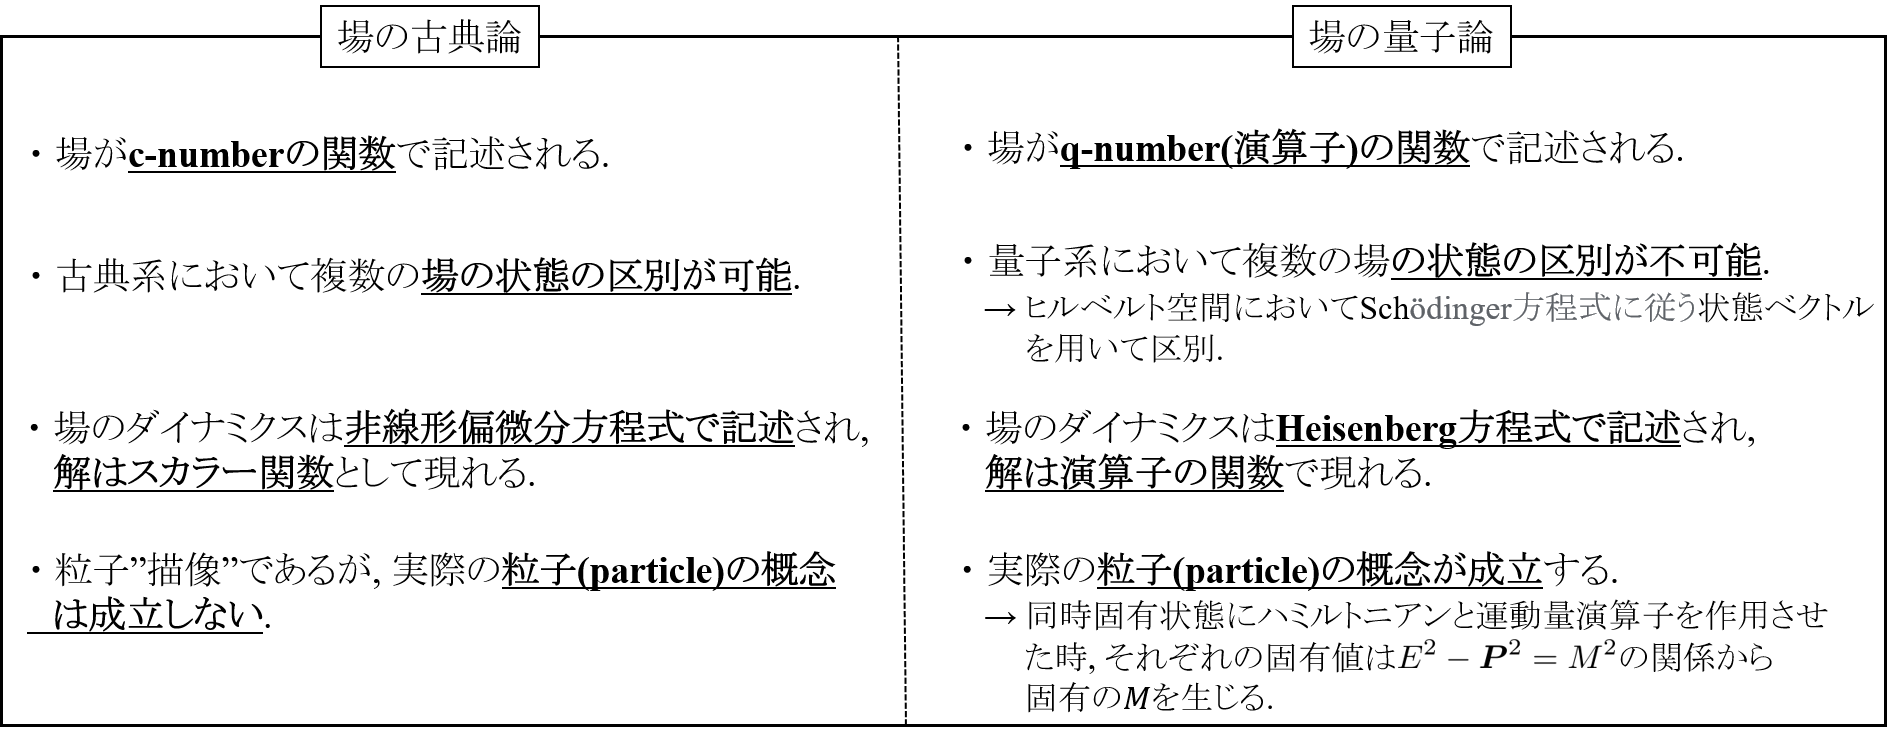
\includegraphics[width=7cm]{figure/fig1.png}
    \caption{}
    \label{fig1}
\end{figure}

では, 量子論ではどうかということを考えると, 不確定性原理から粒子の運動量または位置の変位がゼロに成ることはなく, 粒子の位置と運動は必ず揺らいでいる. 実際, 先のポテンシャルの基底状態であっても
\begin{align}
    E_0=E_{0}^{\text{cl}}+\Delta_0=V(a)+\Delta_0
\end{align}
というように$x=a$付近でエネルギーはゆらぐ. このとき$x=a$まわりで粒子がわずかに振動している場合, ポテンシャル$V(x)$を弱結合展開(weak-coupling expansion)することができる. つまりテイラー展開で
\begin{align}
    V(x)=V(a)+\frac{1}{2}\omega^2(x-a)^2+\frac{1}{3!}\lambda_3(x-a)^3+\frac{1}{4!}\lambda_4(x-a)^4+\cdots
\end{align}
というように調和振動+ゆらぎという形で展開ができる. つまり, $x=a$まわりの振動を記述するのは第1項と第2項であり, それ以降は振動とは関係のないゆらぎの項である. したがって, 各項の波動関数には
\begin{align}
    \lambda_r\braket{(x-a)^r} \ll \omega^2\braket{(x-a)^2}, \qquad r=3,4,\cdots
\end{align}
の関係が成立しており, 同時にエネルギー固有値は
\begin{align}
    e_n=V(a)+\left(n+\frac{1}{2}\right)\hbar\omega+\mathcal{O}(\lambda_r)
\end{align}
というように定まることがわかる. そして基底状態に関して言えば
\begin{align}
    E_0=V(a)+\frac{1}{2}\hbar\omega+\mathcal{O}(\lambda_r)\label{eq:5.9}
\end{align}
というようにweak-couplingを用いて表現でき, 古典論との関わりがよく見て取れる.

実際に量子論において状態の完全な情報は、その波動関数に含まれています。しかし、古典的な解法では、同じ近似式で、基底状態の波動関数の他の特徴も得られます。この基本的な理由は、古典解x=aの周りに局在していても 例えば、その位置期待値は次のように与えられる。





\end{document}
